\documentclass[sigconf]{acmart}
\usepackage{lipsum} % 用于生成示例文本
\settopmatter{printacmref=false} % Removes citation information below abstract
\renewcommand\footnotetextcopyrightpermission[1]{} % removes footnote with conference information in first column
\pagestyle{plain} % removes running headers
\usepackage{booktabs}
\usepackage{graphicx}
\usepackage{adjustbox}
\usepackage{caption}
\usepackage{tabularx}

\title{A Self-Adaptive System in Information Sharing Platform\\
Group 12
}
\author{Guanjie Wang}
\affiliation{%
  \institution{University of Waterloo}
  \city{Waterloo}
  \state{Ontario}
  \country{Canada}\\
  \texttt{t73wang@uwaterloo.ca}
}

\author{Luchen Zhao}
\affiliation{%
  \institution{University of Waterloo}
  \city{Waterloo}
  \state{Ontario}
  \country{Canada}\\
  \texttt{l32zhao@uwaterloo.ca}
}
\begin{document}

\begin{abstract}
Modern software systems, including web services and mobile apps, operate in 
diverse environments with unique configurations. Given the unpredictability 
of these environments, it's impractical to list all options during design. 
Consequently, dynamic runtime planning is essential to determine optimal configurations\cite{FredericksErikM.2019PaOD}. 
Self adaptation offers a structured approach to address operational uncertainties
 like external disruptions, sensor data changes, and shifting user demands, 
 prioritizing formal assurances as the demand for precise, 
 self-adaptive systems grows\cite{ShevtsovStepan2019SACA}. 
 Furthermore, the widespread use of the internet and personal computing devices has
  elevated the demand for accurate and timely information access, 
  requiring existing services to be high-performing, responsive, and fault-tolerant. 
  Adaptive computing meets these requirements, and we've developed a SAFD system 
  based on adaptive computing to dynamically adjust systems in various operational 
  environments while maintaining these high standards.
\end{abstract}

\keywords{Self-Adaptive, MAPE-K}
\maketitle
\pagestyle{plain}

\section{PROBLEM DESCRIPTION}
A high-quality news and information server needs to simultaneously achieve three key attributes: 
high performance,high concurrency, and high availability to ensure a stable user experience 
during different times, seasons, and traffic fluctuations. However, due to variations in 
the number of users, different time points, and network conditions, the server's load may also differ. 
Specifically, the main challenges currently facing the server include two aspects:
\subsection*{1.1 Load Expansion Issue}
When facing a sudden surge in user traffic, the server may exceed its current maximum load capacity, 
potentially causing delays in responding to user requests. This can have a negative impact on the 
server's ability to provide services to users.
\subsection*{1.2 Extended Wait Times}
As the volume of user traffic increases, the waiting time for each user to access the required 
information also significantly increases. This can adversely affect user satisfaction and the 
overall user experience.
\\
\\
Therefore, for solving above challenges news and information service websites(allrecipes, CBC News, etc) 
need to continuously monitor their systems, including but not limited to monitoring CPU usage, 
memory utilization, network request counts, and response rates. 
They should also promptly respond to any issues that occur during server runtime to 
ensure the server's three key attributes and maintain a consistent user experience.
\section{PROBLEM SALUTATION}
To address the previously mentioned issues, we have developed an adaptive 
system using MAPE-K model\cite{IglesiaDidacGilDeLa2015MFTt} designed to enhance server availability, scalability, and reliability, 
thereby reducing the likelihood of network service problems and meeting the "three high"
requirements of the server. Our focus is on introducing a self-adaptive foodlover, 
a carefully crafted information-sharing website that has resolved potential issues 
in previous versions and improved the overall service capabilities of the system.
Below is the system architecture diagram.
\begin{figure}[H]
  \begin{minipage}{0.5\textwidth}
    \centering
    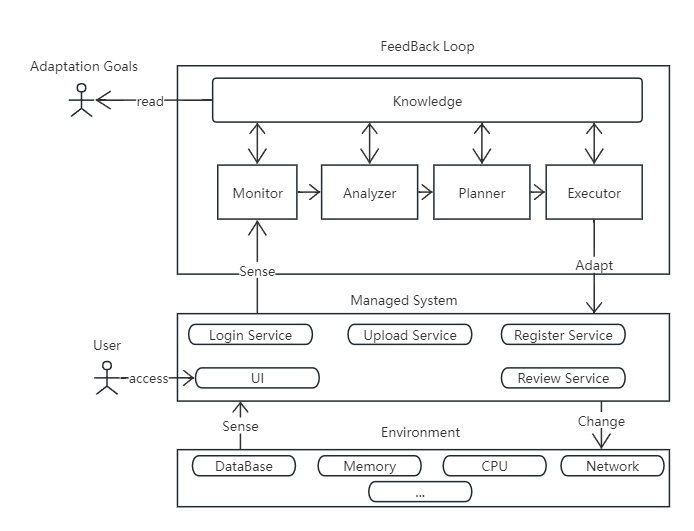
\includegraphics[width=0.8\textwidth]{arch.png}
    \caption{System Architecture Diagram}
    \label{fig:architecture}
  \end{minipage}
\end{figure}
\section{MAPE-K}
\subsection{Monitor}
The purpose of the monitor is to collect the data required for the self-adaptive foodlover system. This data includes crucial metrics such as CPU usage, memory usage, and the network error rate from the server. The monitor plays a vital role in ensuring the system's performance and reliability by continuously gathering information about its resource utilization and error rates.The monitor continually tracks these metrics, providing real-time data to inform the system's adaptive behaviours. By collecting and analyzing this information, the system can proactively respond to changing conditions and ensure that it meets its adaptation goals, providing a seamless and reliable user experience for the self-adaptive Foodlover platform.
\begin{table}[H]
    \adjustbox{max width=0.5\textwidth}{
        \begin{minipage}{0.5\textwidth}
        % 左侧为空白
      \end{minipage}%
          \begin{minipage}{0.5\textwidth}
          \centering
	\begin{tabularx}{\textwidth}{lXX}
		\toprule \textbf{Metrics}
		&  \textbf{Adaptation Goal} & \textbf{Task }  \\
		\midrule
		CPU 
		&  Maintain CPU usage at 85\% 
		& Horizontal increase the pod, compress the PDF file\\
		 Memory & Keep memory usage at 85\% & Horizontal increase the pod
                 compress the PDF file\\
          Error Rate & Keep the error rate below 30\% & Update the LoadBalancer and update the administrator \\
		\bottomrule
	\end{tabularx}
	\caption{System Adaptation Goals}
        \label{fig:adaption}
 \end{minipage}
    }
\end{table}
\subsection{Analyzer}
We will also explore a series of strategies for different adaptation goals, which are detailed in Table 1. Through statistical analysis methods, we can gain a better understanding of the trends and patterns in the monitoring data, providing more precise guidance for the system's adaptability. We will use this data with the utility function to identify potential bottlenecks and performance constraints, as well as possible solutions. This data-driven approach will contribute to improving the user experience and ensuring that the system maintains high performance and availability in a constantly changing environment. By analyzing and optimizing adaptive strategies, we can better meet the needs of different users and applications, delivering superior services. Below is the utility function.
\begin{equation*}
\adjustbox{max width=0.5\textwidth}{
  \begin{minipage}{0.5\textwidth}
    \centering
    % 左侧为空白
  \end{minipage}%
  \begin{minipage}{0.5\textwidth}
    \centering
    U_c = w_{\text{CPU\%}} \cdot p_{\text{CPU\%}} + w_{\text{mem\%}} \cdot p_{\text{mem\%}} + w_{\text{net\_connection\_cnt}} \cdot p_{\text{net\_connection\_cnt}} + w_{\text{error\_cnt}} \cdot p_{\text{error\_cnt}}
  \end{minipage}
}
\end{equation*}

\subsection{Planner}
The utility function value plays a pivotal role in our decision-making process, particularly when it comes to maintaining the server’s “three high” status. This term refers to high availability, high performance, and high security, which are critical attributes for any robust server system. Our goal is to ensure that these three attributes are consistently upheld. To achieve this, we employ a planner that meticulously evaluates various system configurations. Each configuration is assigned a utility value, which is a quantitative measure of its effectiveness in maintaining the “three high” status. Once all configurations have been evaluated and their utility values determined, the planner selects the one with the highest value. This systematic and data-driven approach allows us to optimize our server system effectively, ensuring it consistently delivers high performance, remains readily available, and upholds stringent security standards.

\subsection{Executor}
The executor will perform the optimization which the planner identified to the managed system which is shown in Figure 1, such as: sending the compressed pdf document or horizontally increasing the pod number.
\section{USED TECHNOLOGY}
\begin{table}[H]
    \adjustbox{max width=0.5\textwidth}{
        \begin{minipage}{0.5\textwidth}
        % 左侧为空白
      \end{minipage}%
          \begin{minipage}{0.5\textwidth}
          \centering
	\begin{tabularx}{\textwidth}{lX}
		\toprule \textbf{Technology}
		&  \textbf{Description} \\
		\midrule
		Docker & Service running environment \\
        Python & Data analysis \\
        Flask & BackEnd Services \\
        HTML, CSS, JS & FrontEnd UI \\
        MongoDB or MySQL & Data Storage \\
        MiniKube & Docker Management \\
		\bottomrule
	\end{tabularx}
	\caption{Technology Used}
      \label{fig:Technology}
 \end{minipage}
    }
\end{table}



\section{TIMELINE}
1.	Develop the service on the local machine - 1 week\\
2.	Containerization and monitoring data - 1 week\\
3.	Realize self-optimizing - 2 weeks\\
4.	Integrate adaptation loop and evaluation - 1 week\\
5.	Documentation - 1 week

\bibliographystyle{ACM-Reference-Format}
\bibliography{refs}
\end{document}
